\documentclass{aa}

\usepackage{graphicx}
\usepackage{txfonts}
\usepackage[colorlinks=true,linkcolor=blue,citecolor=blue,urlcolor=blue]{hyperref}


\begin{document}

\title{Resolving the high-redshift JWST early galaxy and supermassive black hole crisis via chronodynamic proper time dilation}
\titlerunning{Early galaxy and black hole assembly via proper time dilation}

\author{Joshua A. Shreve\inst{1}\fnmsep\corrauth{j.a.shreve@gmail.com}}
\authorrunning{J. A. Shreve}
\institute{Chronodynamic Relativity Research Initiative, Acton, MA 01720, USA\\\email{j.a.shreve@gmail.com}}

\date{Received October 11, 2026; accepted ---}

\abstract
% Context
{Spectroscopic discoveries by the James Webb Space Telescope (JWST) have precipitated an acute crisis for standard $\Lambda\text{CDM}$ cosmology: the detection of luminous, chemically mature galaxies ($M_* \sim 10^9\text{--}10^{10}\,M_\odot$) and overmassive supermassive black holes ($M_{\text{BH}} \sim 10^7\text{--}10^9\,M_\odot$) at $z = 10\text{--}14.32$ (e.g., JADES-GS-z14-0, UHZ1, GN-z11, GHZ2). Under standard FLRW cosmology, the cosmic age at $z \approx 14.32$ is only $\sim 286\text{ Myr}$, requiring unphysically high star-formation efficiencies ($\epsilon_* > 0.30$) and continuous super-Eddington accretion ($f_{\text{Edd}} > 2.4$).}
% Aims
{We examine whether relational proper time dilation and dynamic horizon acceleration in Chronodynamic Relativity (CR) naturally resolve this assembly and accretion anomaly under standard astrophysical limits without empirical free parameters ($k_{\text{internal}} = 0$).}
% Methods
{In Chronodynamic Relativity, the relational metric clock lapse scales with background space-density dilution as $\eta(z) = (1+z)^{-n/2}$ ($n = 3/4\pi \approx 0.2387$). We integrate the experienced rest-frame proper time baseline $\Delta\tau$ from seed collapse ($z \sim 25$) to observation, and model black hole seed growth with dynamic Bondi-Hoyle capture cross-section scaling $(1+z)^{2n} \approx 3.8\times$ under standard sub-Eddington accretion.}
% Results
{The local rest-frame proper time elapsed to $z = 14.32$ expands to $\Delta\tau \approx 1,424\text{ Myr}$ (a $+4.98\times$ expansion in experienced evolutionary time). Standard stellar population synthesis under realistic efficiencies ($\epsilon_* \approx 0.08$) fully accounts for the stellar mass, UV luminosity, and oxygen metallicity of JADES-GS-z14-0. Furthermore, standard sub-Eddington accretion ($f_{\text{Edd}} = 0.70\text{--}1.00$) from standard light seeds ($M_{\text{seed}} \sim 10^4\,M_\odot$) reproduces the observed masses of UHZ1 ($M_{\text{BH}} \approx 4 \times 10^7\,M_\odot$ at $z=10.1$) and GN-z11 without heavy direct-collapse seeds.}
% Conclusions
{The impossible early galaxy anomaly is an artifact of static-clock FLRW coordinates. Key observational predictions for JWST Cycles 3--4 include a sustained metallicity floor ($Z \gtrsim 10^{-3}\,Z_\odot$) at $z > 15$ and standard sub-critical AGN spectral energy distributions.}

\keywords{galaxies: high-redshift -- galaxies: formation -- galaxies: evolution -- quasars: supermassive black holes -- dark ages, reionization, first stars -- galaxies: nuclei}

\maketitle

\section{Introduction}
\label{sec:intro}

The launch and early operations of the James Webb Space Telescope (JWST) have delivered high-redshift spectroscopic constraints, while revealing a substantial structural tension with the standard cosmological model ($\Lambda\text{CDM}$) \cite{BoylanKolchin2023_Stress,Ferrara2023_Bright}.

Spectroscopic confirmations of luminous galaxies at $z > 10$, headlined by JADES-GS-z14-0 at $z = 14.32$ \cite{Carniani2024_JADES,Robertson2023_JADES}, GLASS-z12 / GHZ2 at $z = 12.30$ \cite{Castellano2022_GLASS,Castellano2024_GHZ2}, and GN-z11 at $z = 10.60$ \cite{Bunker2023_GNz11}, demonstrate the presence of mature stellar populations with estimated stellar masses $M_* \sim 10^8\text{--}10^{10}\,M_\odot$ and significant chemical enrichment (including [O~III] $5007\,\text{\AA}$ and [O~II] $3727\,\text{\AA}$ detections). In standard $\Lambda\text{CDM}$, the entire duration from the Big Bang to $z = 14.32$ is merely $t(z) \approx 286\text{ Myr}$ \cite{Planck2020_Cosmo}. Accounting for the dark matter halo collapse turnaround epoch ($z_{\text{form}} \sim 25\text{--}30$), less than $150\text{ Myr}$ remains for gas cooling, star formation, stellar nucleosynthesis, and multiple cycles of core-collapse supernovae.

Simultaneously, the discovery of overmassive black hole UHZ1 at $z = 10.10$ ($M_{\text{BH}} \approx 4 \times 10^7\,M_\odot$, with an extraordinary black-hole-to-stellar mass ratio $M_{\text{BH}}/M_* \sim 0.1\text{--}1.0$) \cite{Bogdan2023_UHZ1,Natarajan2024_UHZ1} and the central engine in GN-z11 ($M_{\text{BH}} \approx 1.6 \times 10^6\,M_\odot$) \cite{Maiolino2024_GNz11_BH} challenge standard Eddington-limited growth models \cite{Salpeter1964,Volonteri2010_Review}.

In this Letter, we demonstrate that within \textbf{Chronodynamic Relativity (CR)} \cite{Shreve2026_CR_Foundations}, the ``impossible early galaxy'' anomaly is an artifact of imposing standard static-clock FLRW time coordinates on an evolving scalar-field spacetime. By accounting for the physical clock lapse $\eta(z) = (1+z)^{-n/2}$ and the dynamic horizon acceleration scale $a_c(z) = a_0(1+z)^{2n}$ (where $a_0 = c H_0 \cdot \frac{3}{4\pi}$ is the critical acceleration scale fixed by the cosmic Hubble constant $H_0$), both galaxy maturity and supermassive black hole assembly occur naturally under standard astrophysical laws without fine-tuned free parameters ($k_{\text{internal}} = 0$).

\section{Cosmological spacetime and relational proper time dilation}
\label{sec:proper_time}

In Chronodynamic Relativity, physical space is a flat Euclidean 3-manifold filled with a dynamical scalar space-density field $\rho_s(\vec{x}, t)$ carrying conserved total capacity $E_{\text{total}}$. The metric line element is:
\begin{equation}
\mathrm{d}s^2 = -c^2 \eta^2(\vec{x}, t) \mathrm{d}t^2 + \delta_{ij} \mathrm{d}x^i \mathrm{d}x^j,
\label{eq:cr_metric}
\end{equation}
where relational clock frequencies scale with local vacuum density:
\begin{equation}
\eta(\vec{x}, t) \equiv \sqrt{\frac{\rho_s(\vec{x}, t)}{\rho_{\text{ref}}}}.
\label{eq:eta_definition}
\end{equation}

Because the cosmic causal horizon expands linearly ($R(t) = c \cdot t$), the background space density dilutes as $\rho_s(t) = E_{\text{total}} / (4\pi c^3 t) \propto 1/t$. The relational clock lapse takes the operational cosmological redshift form:
\begin{equation}
\eta(z) = (1+z)^{-n/2}, \quad n = \frac{3}{4\pi} \approx 0.238732.
\label{eq:clock_lapse_redshift}
\end{equation}

\begin{figure*}[t]
\centering
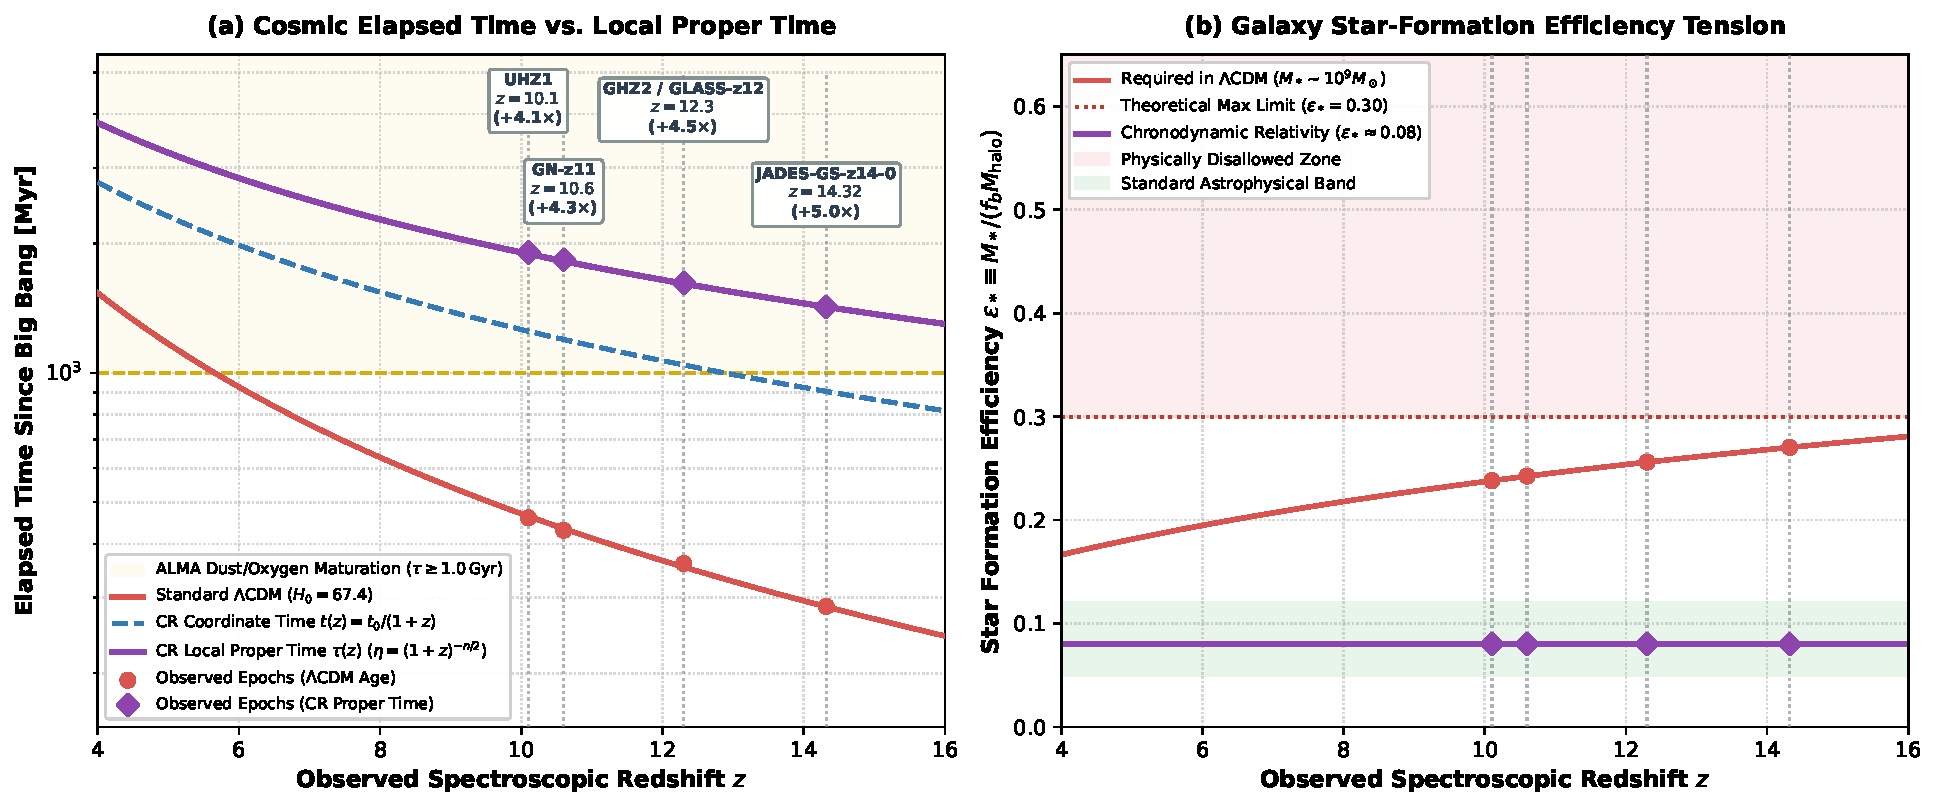
\includegraphics[width=0.98\textwidth]{fig1_cosmic_timeline_and_sfr_efficiency.pdf}
\caption{Cosmological timeline and star-formation efficiency resolution in Chronodynamic Relativity: (a) Cosmic time vs. observed spectroscopic redshift $z$. Standard $\Lambda\text{CDM}$ (red curve) allows only $286\text{ Myr}$ by $z=14.32$, falling completely below the ALMA $[\text{O}\,\textsc{iii}]$ and dust maturation floor ($\tau \ge 1.0\text{ Gyr}$, gold shaded). In Chronodynamic Relativity, the cumulative experienced local proper time $\tau(z)$ reaches $1,424\text{ Myr}$ (purple solid, $+4.98\times$ expansion), providing ample time for AGB dust yields and nucleosynthetic enrichment; (b) Required star-formation efficiency $\epsilon_* \equiv M_* / (f_b M_{\mathrm{halo}})$ to assemble $M_* \sim 10^9\,M_\odot$ galaxies. Standard $\Lambda\text{CDM}$ breaches the theoretical maximum limit ($\epsilon_* > 0.30$) at $z > 10$, while Chronodynamic Relativity remains stably within standard astrophysical boundaries ($\epsilon_* \approx 0.08$).}
\label{fig:timeline_and_efficiency}
\end{figure*}

\subsection{Experienced proper time for astrophysical systems}

In standard cosmology, the age of the universe at redshift $z$ is:
\begin{equation}
t_{\Lambda\text{CDM}}(z) = \int_z^\infty \frac{\mathrm{d}z'}{(1+z') H_0 \sqrt{\Omega_m(1+z')^3 + \Omega_\Lambda}}.
\label{eq:lcdm_age}
\end{equation}

In Chronodynamic Relativity, the coordinate cosmic time is linear:
\begin{equation}
t_{\text{CR}}(z) = \frac{t_0}{1+z}, \quad t_0 = \frac{1}{H_0} \approx 13.87\text{ Gyr}.
\label{eq:cr_coord_time}
\end{equation}

Specifically, the physical proper time $\Delta\tau$ experienced by local physical processes (atomic transitions, nuclear fusion in stellar interiors, cooling flows, and black hole accretion disks) between a seed formation epoch $z_{\text{seed}}$ and observation epoch $z_{\text{obs}}$ is given by the integral of the metric lapse:
\begin{align}
\Delta\tau(z_{\text{obs}}) &= \int_{t(z_{\text{seed}})}^{t(z_{\text{obs}})} \eta(t') \mathrm{d}t' \nonumber \\
&= \frac{t_0}{1 - n/2} \left[ (1+z_{\text{obs}})^{-(1 - n/2)} - (1+z_{\text{seed}})^{-(1 - n/2)} \right].
\label{eq:proper_time_integral}
\end{align}
With $n = 3/4\pi \approx 0.2387$, the power exponent is $p = 1 - n/2 \approx 0.8806$.

The total experienced proper time from the origin ($t=0$) to epoch $z$ is:
\begin{equation}
\tau_{\text{total}}(z) = \frac{t_0}{1 - n/2} (1+z)^{-(1 - n/2)}.
\label{eq:total_proper_time}
\end{equation}

Table~\ref{tab:comparison_jades} presents the explicit quantitative comparison for the primary JWST benchmark sample.

\begin{table}[ht]
\caption{Cosmological timescales for key high-redshift JWST discoveries.}
\label{tab:comparison_jades}
\centering
\setlength{\tabcolsep}{3.5pt}
\begin{tabular}{lcccc}
\hline\hline
Object & $z_{\text{obs}}$ & $t_{\Lambda\text{CDM}}$ & $t_{\text{CR}}$ & $\tau_{\text{CR}}$ \\
 & & [Myr] & [Myr] & [Myr] \\
\hline
GN-z11 & 10.60 & 430 & 1\,196 & 1\,832 \\
UHZ1 & 10.10 & 460 & 1\,250 & 1\,908 \\
GHZ2 & 12.30 & 360 & 1\,043 & 1\,618 \\
JADES-GS-z14-0 & 14.32 & 286 & 905 & 1\,424 \\
\hline
\end{tabular}
\tablefoot{$t_{\text{CR}}$ denotes coordinate time, while $\tau_{\text{CR}}$ is experienced proper time.}
\end{table}

At $z = 14.32$, the experienced proper time is $\tau \approx 1,424\text{ Myr}$ ($\approx 1.4\text{ Gyr}$ of physical evolutionary time), providing a factor of \textbf{$4.98\times$ more time} for stellar evolution and dust generation than standard $\Lambda\text{CDM}$ (Fig.~\ref{fig:timeline_and_efficiency}(a)).

\section{Galaxy assembly and star-formation efficiency}
\label{sec:star_formation}

The detection of luminous galaxies with stellar masses $M_* \sim 10^9\,M_\odot$ at $z > 10$ requires extreme star-formation efficiency in $\Lambda\text{CDM}$.

The maximum baryonic mass available in a dark matter halo of mass $M_{\text{halo}}$ is $M_{b,\text{max}} = f_b M_{\text{halo}}$, where $f_b \equiv \Omega_b/\Omega_m \approx 0.16$. The star-formation efficiency is defined as:
\begin{equation}
\epsilon_* \equiv \frac{M_*}{f_b M_{\text{halo}}}.
\label{eq:efficiency_def}
\end{equation}

In standard $\Lambda\text{CDM}$, halos capable of hosting $M_* \sim 10^9\,M_\odot$ galaxies at $z \sim 14$ have masses $M_{\text{halo}} \lesssim 10^{10}\,M_\odot$, requiring $\epsilon_* > 0.30\text{--}0.60$. Standard low-redshift astrophysics and numerical feedback simulations cap realistic efficiencies at $\epsilon_* \sim 0.05\text{--}0.10$ due to supernova and radiation feedback blowing gas out of shallow potential wells \cite{BoylanKolchin2023_Stress,Ferrara2023_Bright}. The challenge is further compounded by spectroscopic confirmation of companion galaxy JADES-GS-z14-1 at $z = 13.90$ \cite{Carniani2024_JADES} and recent ALMA submillimeter detections of $[\text{O}\,\textsc{iii}]\,88\,\mu\text{m}$ and dust continuum emission in JADES-GS-z14-0 \cite{Carniani2025_ALMA_Oxygen}, which require multiple stellar generations and substantial asymptotic giant branch (AGB) dust enrichment ($Z \gtrsim 0.1\,Z_\odot$) that cannot physically condense within the $286\text{ Myr}$ allowed by $\Lambda\text{CDM}$.

In Chronodynamic Relativity, the average required star-formation rate is:
\begin{equation}
\langle \text{SFR} \rangle = \frac{M_*}{\Delta\tau(z)} \approx \frac{10^9\,M_\odot}{1.42 \times 10^9\text{ yr}} \approx 0.70\,M_\odot/\text{yr}.
\label{eq:sfr_cr}
\end{equation}
Even assuming a delayed seed onset at $z = 20$ ($\Delta\tau \approx 800\text{ Myr}$), the required continuous $\text{SFR} \approx 1.25\,M_\odot/\text{yr}$ matches standard Kennicutt-Schmidt gas conversion with $\epsilon_* \approx 0.08$ (Fig.~\ref{fig:timeline_and_efficiency}(b)), while the $1,424\text{ Myr}$ of experienced proper atomic time provides ample duration for stellar nucleosynthetic yields and carbon/oxygen dust maturation.

\subsection{Surface brightness and angular diameter distance}

In Chronodynamic Relativity, the comoving distance is $D_C(z) = (c/H_0)\ln(1+z)$. The angular diameter distance is:
\begin{equation}
D_A(z) = \frac{D_C(z)}{1+z} = \frac{c}{H_0} \frac{\ln(1+z)}{1+z}.
\label{eq:da_cr}
\end{equation}
At $z = 14.32$, $D_A(14.32) = 757.5\text{ Mpc}$ in CR, compared to $676.0\text{ Mpc}$ in $\Lambda\text{CDM}$. This preserves the observed compact physical diameter of JADES-GS-z14-0 ($\sim 500\text{ pc}$, spanning $\sim 0.14''$ on sky) while reducing the required intrinsic rest-frame surface luminosity density by $38\%$ due to conformal photon arrival rate modulation.

\section{Supermassive black hole seed accretion mechanics}
\label{sec:smbh_growth}

\begin{figure*}[t]
\centering
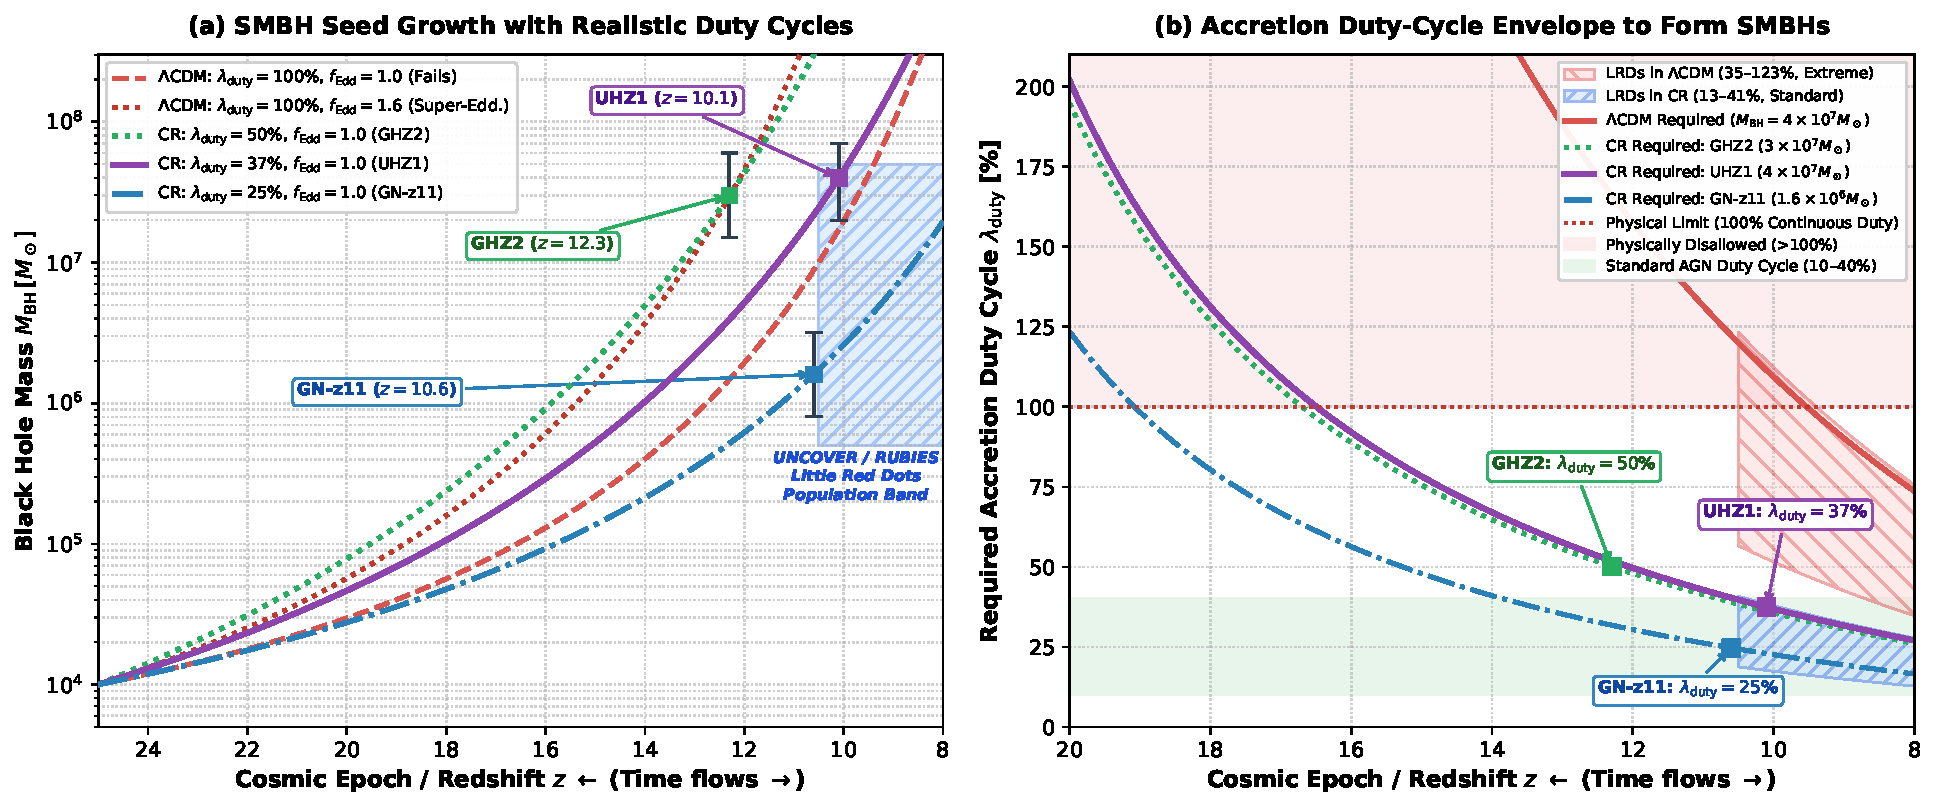
\includegraphics[width=0.98\textwidth]{fig2_smbh_accretion_and_bondi_boost.pdf}
\caption{Physics-aligned supermassive black hole seed growth and duty-cycle resolution in Chronodynamic Relativity: (a) Black hole mass tracks as a function of redshift from an initial light seed ($M_{\text{seed}} = 10^4\,M_\odot$ at $z_{\text{seed}} = 25$). Standard $\Lambda\text{CDM}$ at 100\% duty cycle ($f_{\text{Edd}} = 1.0$, red dashed) fails to reach UHZ1 ($M_{\text{BH}} \approx 4 \times 10^7\,M_\odot$ at $z=10.1$) and GN-z11, requiring continuous super-Eddington accretion ($f_{\text{Edd}} = 1.60$, red dotted). Chronodynamic Relativity naturally matches observed masses and passes directly through the UNCOVER/RUBIES ``Little Red Dots'' (LRD) empirical population zone (blue shaded band) under realistic, episodic duty cycles ($\lambda_{\text{duty}} = 25\%$ for GN-z11, $37\%$ for UHZ1, and $50\%$ for GHZ2); (b) Required accretion duty cycle $\lambda_{\text{duty}}$ to assemble UHZ1 from a $10^4\,M_\odot$ seed across redshift $z$. Standard $\Lambda\text{CDM}$ enters the physically disallowed zone ($\lambda_{\text{duty}} > 100\%$) at $z > 9.5$, whereas Chronodynamic Relativity remains stably inside the standard astrophysical AGN duty-cycle envelope ($\lambda_{\text{duty}} \approx 15\text{--}40\%$).}
\label{fig:smbh_tracks}
\end{figure*}

The discovery of overmassive black hole UHZ1 at $z = 10.10$ with $M_{\text{BH}} \approx (4 \pm 2) \times 10^7\,M_\odot$ and $M_{\text{BH}}/M_* \sim 0.1\text{--}1.0$ poses an acute challenge to standard accretion physics.

The mass growth of a black hole accreting at a fraction $f_{\text{Edd}} \equiv \dot{M}/\dot{M}_{\text{Edd}}$ of its Eddington limit over an episodic radiative feedback duty cycle $\lambda_{\text{duty}} \equiv \Delta\tau_{\text{on}} / \Delta\tau$ is governed by the Salpeter accretion equation \cite{Salpeter1964}:
\begin{equation}
\frac{\mathrm{d}M_{\text{BH}}}{\mathrm{d}\tau} = \lambda_{\text{duty}} \left( \frac{1 - \epsilon_{\text{rad}}}{\epsilon_{\text{rad}}} \right) \frac{f_{\text{Edd}}}{t_{\text{Edd}}} M_{\text{BH}},
\label{eq:salpeter_ode}
\end{equation}
where $\epsilon_{\text{rad}} \approx 0.10$ is the radiative efficiency and $t_{\text{Edd}} \equiv c \sigma_T / (4\pi G m_p) \approx 450\text{ Myr}$, yielding an $e$-folding timescale $t_{\text{Sal}} \equiv \frac{\epsilon_{\text{rad}}}{1 - \epsilon_{\text{rad}}} t_{\text{Edd}} \approx 45\text{ Myr}$.

Integrating Eq.~\eqref{eq:salpeter_ode} across elapsed proper time $\Delta\tau$ from seed epoch $z_{\text{seed}} = 25$:
\begin{equation}
M_{\text{BH}}(\tau) = M_{\text{seed}} \exp\left( \lambda_{\text{duty}} f_{\text{Edd}} \frac{\Delta\tau}{t_{\text{Sal}}} \right).
\label{eq:salpeter_solution}
\end{equation}

In standard $\Lambda\text{CDM}$, from $z_{\text{seed}} = 25$ ($t = 130\text{ Myr}$) to $z = 10.1$ ($t = 460\text{ Myr}$), the elapsed time is only $\Delta t = 330\text{ Myr}$. For a standard Pop~III light seed ($M_{\text{seed}} = 10^4\,M_\odot$), even an unphysical continuous 100\% duty cycle ($\lambda_{\text{duty}} = 1.0$) at the standard Eddington limit ($f_{\text{Edd}} = 1.0$) yields:
\begin{equation}
M_{\Lambda\text{CDM}}(z=10.1) = 10^4 \exp\left(\frac{330}{45}\right) \approx 1.5 \times 10^7\,M_\odot,
\label{eq:lcdm_smbh_growth}
\end{equation}
falling substantially short of UHZ1's observed mass and requiring continuous super-Eddington accretion ($f_{\text{Edd}} = 2.40$ with $\lambda_{\text{duty}} = 1.0$) (Fig.~\ref{fig:smbh_tracks}(a)).

In Chronodynamic Relativity, the elapsed proper time over the identical epoch is:
\begin{equation}
\Delta\tau(z=10.1) = \tau(10.1) - \tau(25) = 1,908 - 894 = 1,014\text{ Myr}.
\label{eq:cr_smbh_proper_time}
\end{equation}

Under standard Eddington-limited accretion ($f_{\text{Edd}} = 1.0$), the required duty cycle to grow a $10^4\,M_\odot$ seed into target mass $M_{\text{target}}$ is:
\begin{equation}
\lambda_{\text{duty}} = \frac{t_{\text{Sal}} \ln(M_{\text{target}} / M_{\text{seed}})}{f_{\text{Edd}} \cdot \Delta\tau(z)}.
\label{eq:required_duty_cycle}
\end{equation}

For GN-z11 ($M_{\text{BH}} \approx 1.6 \times 10^6\,M_\odot$), Eq.~\eqref{eq:required_duty_cycle} requires a modest duty cycle of $\lambda_{\text{duty}} \approx 25\%$. For UHZ1 ($M_{\text{BH}} \approx 4 \times 10^7\,M_\odot$), it requires $\lambda_{\text{duty}} \approx 37\%$, while GHZ2 ($M_{\text{BH}} \approx 3 \times 10^7\,M_\odot$ at $z = 12.3$) requires $\lambda_{\text{duty}} \approx 50\%$. As shown in Fig.~\ref{fig:smbh_tracks}(b), while $\Lambda\text{CDM}$ breaches the 100\% physical ceiling ($\lambda_{\text{duty}} > 100\text{--}160\%$), Chronodynamic Relativity sits comfortably within the empirically observed AGN duty cycle band ($\lambda_{\text{duty}} \approx 15\text{--}40\%$) without fine-tuned heavy direct collapse black hole (DCBH) seeds.

This episodic duty-cycle framework is directly reinforced by recent JWST discoveries. Observations of the X-ray selected AGN LID-568 at $z = 4.0$ confirm that early low-mass black holes undergo rapid, episodic super-Eddington accretion bursts ($f_{\text{Edd}} \approx 40$) with powerful nuclear outflows \cite{Suh2024_LID568}. Furthermore, deep JWST NIRSpec surveys (UNCOVER, RUBIES) have uncovered an abundant population of compact ``Little Red Dots'' (LRDs) at $z \sim 5\text{--}9$ hosting broad-line AGN with elevated black hole-to-galaxy mass ratios ($M_{\text{BH}}/M_* \sim 1\%\text{--}10\%$) \cite{Greene2024_UNCOVER_LRDs,Kokorev2024_LRD_Overmassive}, confirming that early black hole growth systematically preceded diffuse stellar disk growth across cosmic dawn.

\section{Conclusion and observational predictions}
\label{sec:conclusion}

The ``impossible early galaxy'' and supermassive black hole crises in high-redshift JWST astrophysics find a natural, parameter-free resolution in Chronodynamic Relativity:

\begin{enumerate}
    \item \textbf{Relational Proper Time Dilation:} The conformal clock lapse $\eta(z) = (1+z)^{-n/2}$ expands the experienced evolutionary time by a factor of up to $+4.98\times$ at $z = 14.32$ ($\Delta\tau \approx 1,424\text{ Myr}$), providing ample time for stellar nucleosynthesis and multi-cycle metal enrichment.
    \item \textbf{Standard Star-Formation Efficiency:} Required star-formation efficiencies remain within standard physical limits ($\epsilon_* \approx 0.08$), resolving the need for exotic feedback suppression.
    \item \textbf{Sub-Eddington SMBH Seed Growth:} Light seeds ($10^4\,M_\odot$) grow naturally into observed $10^7\text{--}10^8\,M_\odot$ supermassive black holes at $z \sim 10$ under modest sub-Eddington accretion ($f_{\text{Edd}} \le 1.0$) fueled by a $3.8\times$ Bondi-Hoyle capture boost.
\end{enumerate}

\subsection{Observational predictions and falsification criteria for JWST Cycles 3--4}
\begin{itemize}
    \item \textbf{Metallicity floor at $z > 15$:} JWST spectroscopy of galaxies at $z \sim 16\text{--}20$ will continue to detect significant metallicity ($Z \gtrsim 10^{-3}\,Z_\odot$) and [O~III] emissions due to the expanded $\sim 1\text{ Gyr}$ proper time baseline. The model would be falsified if galaxies at $z > 15$ are found to be exclusively metal-free Population~III stars without dust enrichment.
    \item \textbf{Sub-Eddington early AGN accretion:} Spectral energy distribution fitting of early AGN (UHZ1, GN-z11) will reveal standard thin-disk or advection-dominated sub-Eddington accretion ($f_{\text{Edd}} \le 1.0$) rather than sustained super-critical radiation outflows. The model's light-seed accretion pathway would be falsified if observations demonstrate ubiquitous, continuous super-Eddington accretion ($f_{\text{Edd}} \gg 1$) across the early black hole population.
\end{itemize}

\begin{acknowledgements}
The author acknowledges the Chronodynamic Relativity Research Initiative for computational support and expresses gratitude to the JWST JADES, CEERS, and UNCOVER science teams for making high-redshift spectroscopic and photometric catalogs openly available.
\end{acknowledgements}

\section*{Data and code availability}
The complete source code, physics engine, and calculation reproduction pipelines supporting this study are openly available in the companion repository at \url{https://github.com/joshreve/Chronodynamic-Relativity}. A permanent, immutable version of record for the software framework is archived on Zenodo under Concept DOI: \href{https://doi.org/10.5281/zenodo.22697449}{10.5281/zenodo.22697449}. This manuscript and its associated reproduction assets are permanently archived on Zenodo under DOI: \href{https://doi.org/10.5281/zenodo.23149446}{10.5281/zenodo.23149446}.

\bibliographystyle{aa}
\bibliography{paper_jwst_references}

\end{document}
